% This is samplepaper.tex, a sample chapter demonstrating the
% LLNCS macro package for Springer Computer Science proceedings;
% Version 2.20 of 2017/10/04
%
\documentclass[runningheads]{llncs}
%
\usepackage{graphicx}
\usepackage{amsmath}
% Used for displaying a sample figure. If possible, figure files should
% be included in EPS format.
%
% If you use the hyperref package, please uncomment the following line
% to display URLs in blue roman font according to Springer's eBook style:
% \renewcommand\UrlFont{\color{blue}\rmfamily}

\begin{document}
%
\title{Conversational Task Agent}
%
%\titlerunning{Abbreviated paper title}
% If the paper title is too long for the running head, you can set
% an abbreviated paper title here
%
\author{Guilherme Fernandes\inst{1}\orcidID{60045} \and
Ricardo Silva\inst{1}\orcidID{60559} \and
Vladyslav Mikytiv\inst{1}\orcidID{60735}}
%
\authorrunning{user204 et al.}
% First names are abbreviated in the running head.
% If there are more than two authors, 'et al.' is used.
%
\institute{NOVA School Of Science and Technology}
%
\maketitle              % typeset the header of the contribution
%
\begin{abstract}
Our project focuses on creating an adaptive taskbot tailored specifically for guiding users through cooking tasks. This taskbot will utilize artificial intelligence and natural language processing to interact with users, understanding their progress and constraints in real-time. Whether it's baking a birthday cake or preparing a gourmet meal, the taskbot will dynamically adjust instructions based on the ingredients and cooking tools available to the user. In instances where users encounter obstacles, such as running out of ingredients or lacking specific utensils, the taskbot will intelligently adapt the recipe, offering alternative ingredient substitutions or equipment alternatives to ensure successful completion of the dish. By providing personalised guidance that accommodates diverse cooking scenarios, our taskbot aims to enhance the culinary experience, empowering users to overcome challenges and achieve culinary success with confidence. 

\keywords{Taskbot  \and Word embedding \and Natural Language Processing}
\end{abstract}
%
%
%
\section{Introduction}
In recent years, word embedding has emerged as a cornerstone technology in the field of artificial intelligence, revolutionising natural language processing (NLP) tasks. This transformative approach to representing words as dense vectors in continuous vector spaces has garnered significant attention and acclaim within the AI community. The rise of word embedding has been marked by its progression from conventional methods to the creation of sophisticated models capable of capturing intricate semantic connections among words.

The inception of word embedding can be traced back to the early 2000s when researchers began exploring methods to overcome the limitations of traditional vector space models, such as bag-of-words and one-hot encoding. These initial efforts paved the way for more advanced approaches that would later reshape the field of natural language processing (NLP).

However, it wasn't until the introduction of groundbreaking techniques like Word2Vec by Mikolov et al. in 2013 and GloVe (Global Vectors for Word Representation) by Pennington et al. in 2014 that word embedding started to gain widespread attention and adoption. These models introduced novel methodologies for learning distributed representations of words based on large corpora of text, capturing intricate semantic nuances and relationships.

The allure of word embedding lies in its ability to encode semantic meaning into dense vector representations, enabling machines to understand language in a more nuanced and contextually rich manner.

The project aims to utilize embedding algorithms and large language models to develop a dialog manager between users and the taskbot. This manager will execute user requests and guide them through processes, particularly in cooking recipes, with adaptability. Leveraging a dataset containing recipes data, including ingredients, procedural steps, and difficulty levels, we utilize OpenSearch indexing to efficiently retrieve information for user queries.


\section{Algorithms and Implementation}
\subsection{Search and Indexing}
We must implement a search index of complex manual tasks in order to allow our system to retrieve relevant information about the tasks.

\begin{figure}[htbp]
    \center
    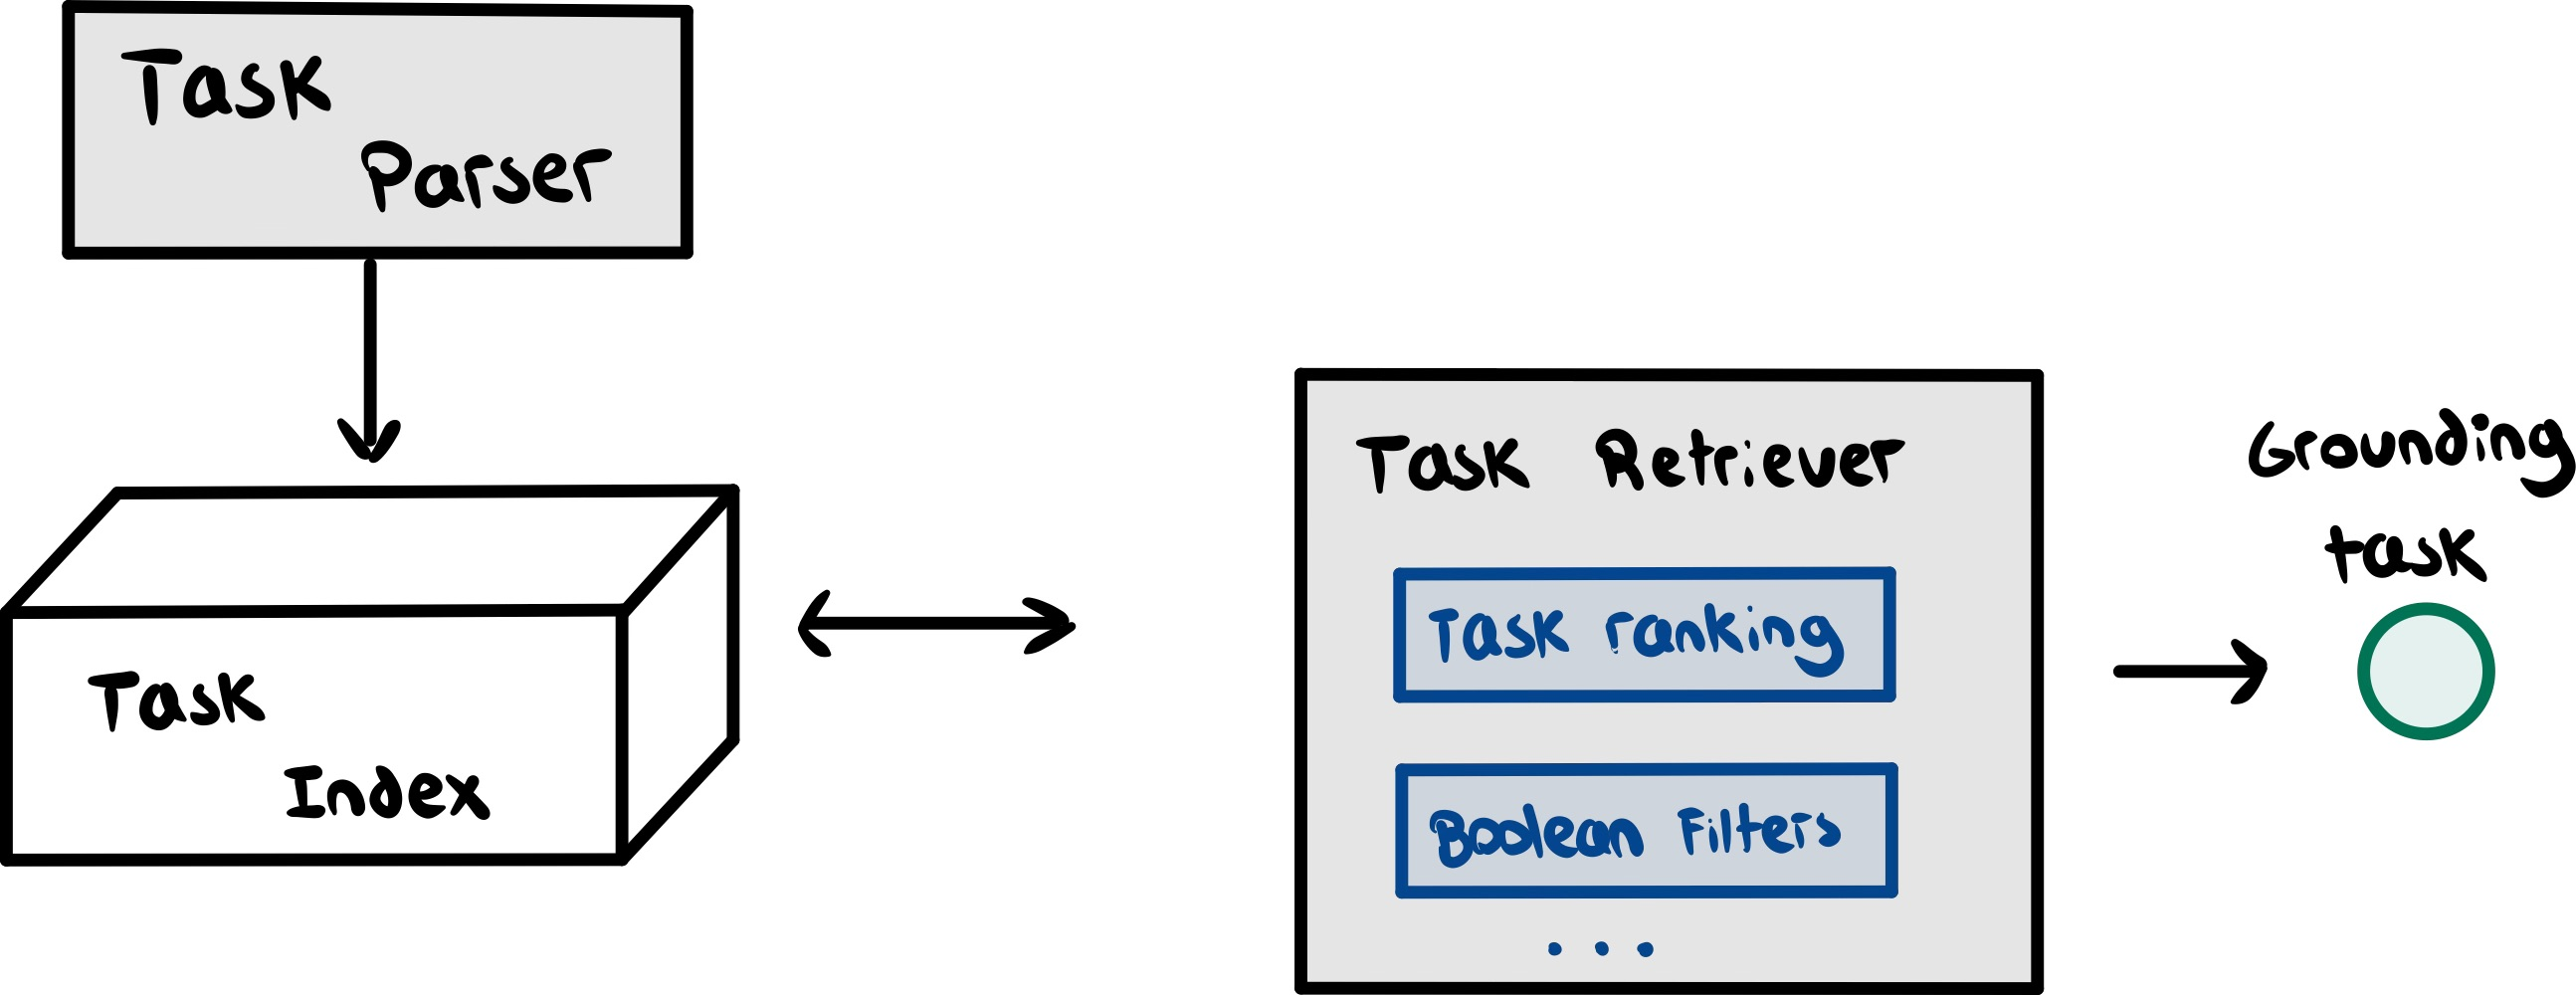
\includegraphics[scale=0.15]{images/task_retriever.jpg}
    \caption{After dependencies removal}
\end{figure}

We must parse the data from the dataset which is a JSON file. We do that while we populate our indexes in OpenSearch. For each recipe we parse the JSON and send the relevant informations to the index mapping that was created. We introduce a set of mappings tailored to effectively index recipe data and they are the following:
\begin{table}[htbp]
\centering
\setlength{\abovecaptionskip}{10pt} % Adjust the spacing here
\begin{tabular}{|c|c|}
\hline
\textbf{Field} & \textbf{Data Type} \\ \hline
recipeJson & object \\ \hline
recipeName & text \\ \hline
prepTimeMinutes & integer \\ \hline
cookTimeMinutes & integer \\ \hline
totalTimeMinutes & integer \\ \hline
difficultyLevel & keyword \\ \hline
images & array of text \\ \hline
servings & float \\ \hline
videos & array of object \\ \hline
tools & array of text \\ \hline
cuisines & array of text \\ \hline
courses & array of text \\ \hline
diets & array of text \\ \hline
stepsEmbedding & \text{knn\_vector} \\ \hline
sentenceEmbedding & \text{knn\_vector} \\ \hline
\end{tabular}
\caption{Mappings for Indexing Recipe Data}
\label{tab:mappings}
\end{table}

\section{Evaluation}
\subsection{Dataset Description}
Please note that the first paragraph of a section or subsection is
not indented. The first paragraph that follows a table, figure,
equation etc. does not need an indent, either.

Subsequent paragraphs, however, are indented.

\subsubsection{Sample Heading (Third Level)} Only two levels of
headings should be numbered. Lower level headings remain unnumbered;
they are formatted as run-in headings.

\paragraph{Sample Heading (Fourth Level)}
The contribution should contain no more than four levels of
headings. Table~\ref{tab1} gives a summary of all heading levels.

\begin{table}
\caption{Table captions should be placed above the
tables.}\label{tab1}
\begin{tabular}{|l|l|l|}
\hline
Heading level &  Example & Font size and style\\
\hline
Title (centered) &  {\Large\bfseries Lecture Notes} & 14 point, bold\\
1st-level heading &  {\large\bfseries 1 Introduction} & 12 point, bold\\
2nd-level heading & {\bfseries 2.1 Printing Area} & 10 point, bold\\
3rd-level heading & {\bfseries Run-in Heading in Bold.} Text follows & 10 point, bold\\
4th-level heading & {\itshape Lowest Level Heading.} Text follows & 10 point, italic\\
\hline
\end{tabular}
\end{table}


\noindent Displayed equations are centered and set on a separate
line.
\begin{equation}
x + y = z
\end{equation}
Please try to avoid rasterized images for line-art diagrams and
schemas. Whenever possible, use vector graphics instead (see
Fig.~\ref{fig1}).

\begin{figure}
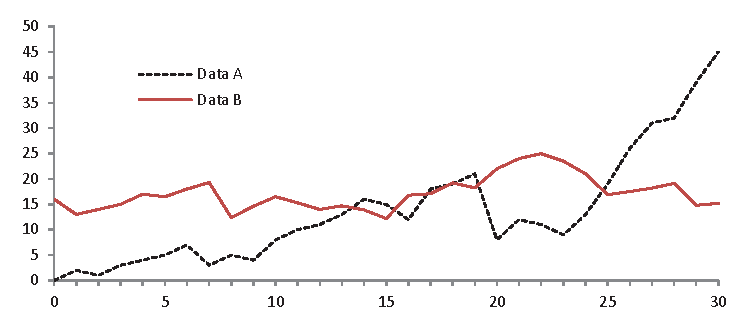
\includegraphics[width=\textwidth]{fig1.eps}
\caption{A figure caption is always placed below the illustration.
Please note that short captions are centered, while long ones are
justified by the macro package automatically.} \label{fig1}
\end{figure}

\begin{theorem}
This is a sample theorem. The run-in heading is set in bold, while
the following text appears in italics. Definitions, lemmas,
propositions, and corollaries are styled the same way.
\end{theorem}
%
% the environments 'definition', 'lemma', 'proposition', 'corollary',
% 'remark', and 'example' are defined in the LLNCS documentclass as well.
%
\begin{proof}
Proofs, examples, and remarks have the initial word in italics,
while the following text appears in normal font.
\end{proof}
For citations of references, we prefer the use of square brackets
and consecutive numbers. Citations using labels or the author/year
convention are also acceptable. The following bibliography provides
a sample reference list with entries for journal
articles~\cite{ref_article1}, an LNCS chapter~\cite{ref_lncs1}, a
book~\cite{ref_book1}, proceedings without editors~\cite{ref_proc1},
and a homepage~\cite{ref_url1}. Multiple citations are grouped
\cite{ref_article1,ref_lncs1,ref_book1},
\cite{ref_article1,ref_book1,ref_proc1,ref_url1}.
%
% ---- Bibliography ----
%
% BibTeX users should specify bibliography style 'splncs04'.
% References will then be sorted and formatted in the correct style.
%
% \bibliographystyle{splncs04}
% \bibliography{mybibliography}
%
\begin{thebibliography}{8}
\bibitem{ref_article1}
Author, F.: Article title. Journal \textbf{2}(5), 99--110 (2016)

\bibitem{ref_lncs1}
Author, F., Author, S.: Title of a proceedings paper. In: Editor,
F., Editor, S. (eds.) CONFERENCE 2016, LNCS, vol. 9999, pp. 1--13.
Springer, Heidelberg (2016). \doi{10.10007/1234567890}

\bibitem{ref_book1}
Author, F., Author, S., Author, T.: Book title. 2nd edn. Publisher,
Location (1999)

\bibitem{ref_proc1}
Author, A.-B.: Contribution title. In: 9th International Proceedings
on Proceedings, pp. 1--2. Publisher, Location (2010)

\bibitem{ref_url1}
LNCS Homepage, \url{http://www.springer.com/lncs}. Last accessed 4
Oct 2017
\end{thebibliography}
\end{document}
